\documentclass[a4paper,10pt,ngerman]{scrartcl}
\usepackage{babel}
\usepackage[T1]{fontenc}
\usepackage[utf8x]{inputenc}
\usepackage[a4paper,margin=2.5cm,footskip=0.5cm]{geometry}
\usepackage{wrapfig}

% Die nächsten vier Felder bitte anpassen:
\newcommand{\Aufgabe}{Aufgabe 4: Würfelglück } % Aufgabennummer und Aufgabennamen angeben
\newcommand{\TeamId}{?????}                       % Team-ID aus dem PMS angeben
\newcommand{\TeamName}{234bcd}                 % Team-Namen angeben
\newcommand{\Namen}{Michael Köhler}           % Namen der Bearbeiter/-innen dieser Aufgabe angeben
 
% Kopf- und Fußzeilen
\usepackage{scrlayer-scrpage, lastpage}
\setkomafont{pageheadfoot}{\large\textrm}
\lohead{\Aufgabe}
\rohead{Team-ID: \TeamId}
\cfoot*{\thepage{}/\pageref{LastPage}}

% Position des Titels
\usepackage{titling}
\setlength{\droptitle}{-1.0cm}

% Für mathematische Befehle und Symbole
\usepackage{amsmath}
\usepackage{amssymb}

% Für Bilder
\usepackage{graphicx}
\graphicspath{ {./images/} }

% Für Algorithmen
\usepackage{algpseudocode}

% Für Quelltext

\usepackage{listings}
\usepackage{color}
\definecolor{mygreen}{rgb}{0,0.6,0}
\definecolor{mygray}{rgb}{0.5,0.5,0.5}
\definecolor{mymauve}{rgb}{0.58,0,0.82}
 \definecolor{cloudwhite}{rgb}{0.225, 0.225, 0.204} 
\definecolor{red}{rgb}{0.4,0,0} 
\definecolor{blue}{rgb}{0,0,0.6}
\definecolor{green}{rgb}{0,0.6,0}
\definecolor{cyan}{rgb}{0.0,0.6,0.6}
\lstset{
language=csh,
basicstyle=\footnotesize\ttfamily,
numbers=left,
numberstyle=\tiny,
numbersep=5pt,
tabsize=2,
extendedchars=true,
breaklines=true,
frame=tb,
showspaces=false,
showtabs=false,
xleftmargin=17pt,
framexleftmargin=17pt,
framexrightmargin=5pt,
framexbottommargin=4pt,
showstringspaces=false,
% confing for comments
commentstyle=\color{green},
morecomment=[l]{//}, 
morecomment=[s]{/*}{*/}, 
% keywords for classes
morekeywords={  List, Program,GameResult,MatchUp,Player,Random },
keywordstyle=\color{cyan},
identifierstyle=\color{cloudwhite},
% keywords for types
emph={int,char,double,float,unsigned,void,bool,var,string,private,static,new,class,using},
emphstyle={\color{blue}},
% other keywords to highlight
classoffset=1, 
otherkeywords={throw},
morekeywords={throw},
keywordstyle=\color{mymauve},
classoffset=0,
% style for strings
stringstyle=\color{red}\ttfamily,
}


% Diese beiden Pakete müssen zuletzt geladen werden
%\usepackage{hyperref} % Anklickbare Links im Dokument
\usepackage{cleveref}

% Daten für die Titelseite
\title{\textbf{\Huge\Aufgabe}}
\author{\LARGE Team-ID: \LARGE \TeamId \\\\
	    \LARGE Team-Name: \LARGE \TeamName \\\\
	    \LARGE Bearbeiter*innen dieser Aufgabe: \\ 
	    \LARGE \Namen\\\\}
\date{\LARGE\today}


\begin{document}


\maketitle
\tableofcontents

\vspace{0.5cm}

%\textbf{Anleitung:} Trage oben in den Zeilen 8 bis 11 die Aufgabennummer, die Team-ID, den Team-Namen und alle Bearbeiter/-innen dieser Aufgabe mit Vor- und Nachnamen ein.
%Vergiss nicht, auch den Aufgabennamen anzupassen (statt "`\LaTeX-Dokument"')!

%Dann kannst du dieses Dokument mit deiner \LaTeX-Umgebung übersetzen.

%Die Texte, die hier bereits stehen, geben ein paar Hinweise zur
%Einsendung. Du solltest sie aber in deiner Einsendung wieder entfernen!


\section{Lösungsidee}
%Die Idee der Lösung sollte hieraus vollkommen ersichtlich werden, ohne dass auf die eigentliche Implementierung Bezug genommen wird.
Für diese Aufgabe muss man wissen, dass Digitalbilder aus vielen Bildpunkten (Pixeln) bestehen, die jeweils eine bestimmte Farbe haben. Wenn man ein Digitalbild ausreichend vergrößert betrachtet, kann man die einzelnen Pixel erkennen. Hier ist ein vergrößerter Ausschnitt aus einem der Beispielbilder für diese Aufgabe (Kontrast ein wenig erhöht): \\
\begin{wrapfigure}{l}{0.5\textwidth} 
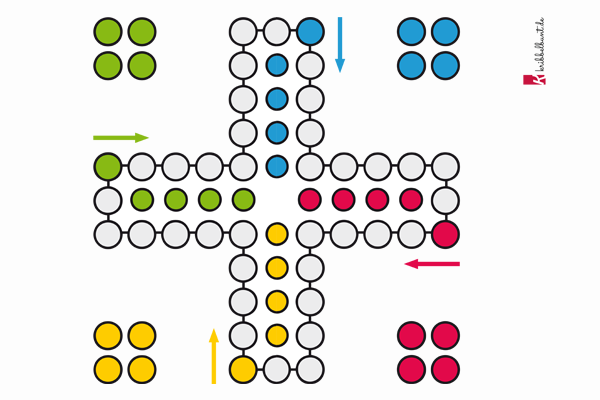
\includegraphics[width=0.5\textwidth]{mensch-aergere-dich-nicht-spielfeld}
\centering
\caption{Spielbrett}
\end{wrapfigure}Bei genauem Hinsehen fällt auf, dass im oberen Bereich des Ausschnittes jedes Pixel eine leicht andere Farbe hat, während unten immer vier Pixel die gleiche Farbe haben. 
Dies sind die Rhinozelfantenschuppen. 
\section{Umsetzung}
%Hier wird kurz erläutert, wie die Lösungsidee im Programm tatsächlich umgesetzt wurde. Hier können auch Implementierungsdetails erwähnt werden.
Die Lösungsidee wird in Python implementiert. Die Python Imaging Library (PIL) stellt viele Funktionen zur Bildverar- beitung zur Verfügung. Damit funktionieren das Öffnen und 
Speichern des Bildes und der Zugriff auf die Pixeldaten sehr einfach. Wir importieren dazu das Modul Image der PIL. Mithilfe zweier ineinander geschachtelter For-Schleifen 
werden alle Pixel einzeln betrachtet. Immer wenn ein Pixel die gleiche Farbe hat wie eines seiner Nachbarpixel, färben wir beide Pixel weiß. Da bei dieser Aufgabe alle Pixel weiß gefärbt werden sollen, die zu einem Rhinozelfant gehören könnten, müssen wir aufpassen, dass wir nicht direkt ein Pixel im Bild weiß färben, wenn wir sehen, dass es einen gleichfarbigen Nachbarn 
gibt. Sonst kann es passieren, dass wir bei den anderen benachbarten Pixeln nicht mehr wissen, welche Farbe das aktuelle Pixel ursprünglich hatte. Dieses Problem wird 
gelöst, indem nicht die Pixel im Originalbild weiß gefärbt werden, sondern in einer Kopie des Bildes ('ausgabebild'). Dadurch können wir im Originalbild immer alle Pixel in ihrer 
ursprünglichen Farbe vergleichen. Zu guter Letzt wird das Ausgabebild wieder in eine Datei 
gespeichert. 
\section{Beispiele}
%Genügend Beispiele einbinden! Die Beispiele von der BwInf-Webseite sollten hier diskutiert werden, aber auch eigene Beispiele sind sehr gut – besonders wenn sie Spezialfälle abdecken. Aber bitte nicht 30 Seiten Programmausgabe hier einfügen!
Wir rufen das Programm für zwei der Beispieldateien auf und zeigen jeweils das resultierende Bild in verkleinerter Darstellung: 
\section{Quellcode}
%Unwichtige Teile des Programms sollen hier nicht abgedruckt werden. Dieser Teil sollte nicht mehr als 2–3 Seiten umfassen, maximal 10.
Beispiel-Code:
\begin{lstlisting}
static void Main(string[] args)
        {
//test Comment!
            List<Player> players = SetPlayers(args);
            List<MatchUps> matchups = CreateMatchups(players);
            List<GameResults> gameresults = PlayGames(matchups);
            RankPlayers(gameresults);
	 Console.WriteLine("Test string");
            
        }
\end{lstlisting}
Program.cs:
\lstinputlisting{DiceCompare/Program.cs}

\end{document}
